\documentclass[aspectratio=169, 10pt]{beamer}

\usetheme[progressbar=frametitle]{metropolis}
\usepackage{appendixnumberbeamer}

\usepackage{booktabs}
\usepackage[scale=2]{ccicons}

\usepackage{pgfplots}
\usepgfplotslibrary{dateplot}

\usepackage{xspace}
\newcommand{\themename}{\textbf{\textsc{metropolis}}\xspace}

\title{Annotation Quality}

% \subtitle{A modern beamer theme}
% \date{\today}
\date{}

\author{Yisong Tang, Ali Doğukan Sven, Karel Štícha}

% \institute{Center for modern beamer themes}
% \titlegraphic{\hfill\includegraphics[height=1.5cm]{logo.pdf}}

\begin{document}

\maketitle

\begin{frame}{Precision of Temporal Annotations}
\begin{itemize}
    \item We analyzed the \textbf{duration} of overlapping annotations to assess precision.
    \item High variability in duration (\( \text{SD} \approx 10 \) sec, \( \text{IQR} > 20 \) sec), annotators agreed on the number of distinct sound events in 94.7\% of cases.
    \item Results: Strong agreement on if something happened, but not on for how long it happened.
\end{itemize}
\end{frame}



\begin{frame}{Similarity of textual annotations}
    \begin{itemize}
        \item \textbf{Text length}
            \begin{itemize}
                \item High variation (SD = 4.33 words), indicating a high variability in the level of detail.
                \item Most annotators prefer short, succinct descriptions.
            \end{itemize}

        \vspace{.5cm}
        \item \textbf{Cosine Similarity}
            \begin{itemize}
                \item Inter-quartile range: -0.03 to 0.14.
                \item Annotators use frequently different words, and sometimes even contradict each other.
            \end{itemize}        
    \end{itemize}
\end{frame}




\begin{frame}{Frequency and Detail of Annotations)}
    \begin{itemize}
        \item Each file had: 3.99 annotations, and 3.72 distinct sound events.
        \item Some files understandably contain only one sound event.
        \end{itemize}

        
        \item \textbf{Annotation Length as Proxy for Detail}
        \begin{itemize}
            \item Median length = 7 words, however Over 1000 annotations contain only one word
            \item Positively skewed distribution → Most annotations are brief, a few are long and detailed.
        \end{itemize}
\begin{figure}[h]
    \centering
    %Elbow+Silhouette plot
    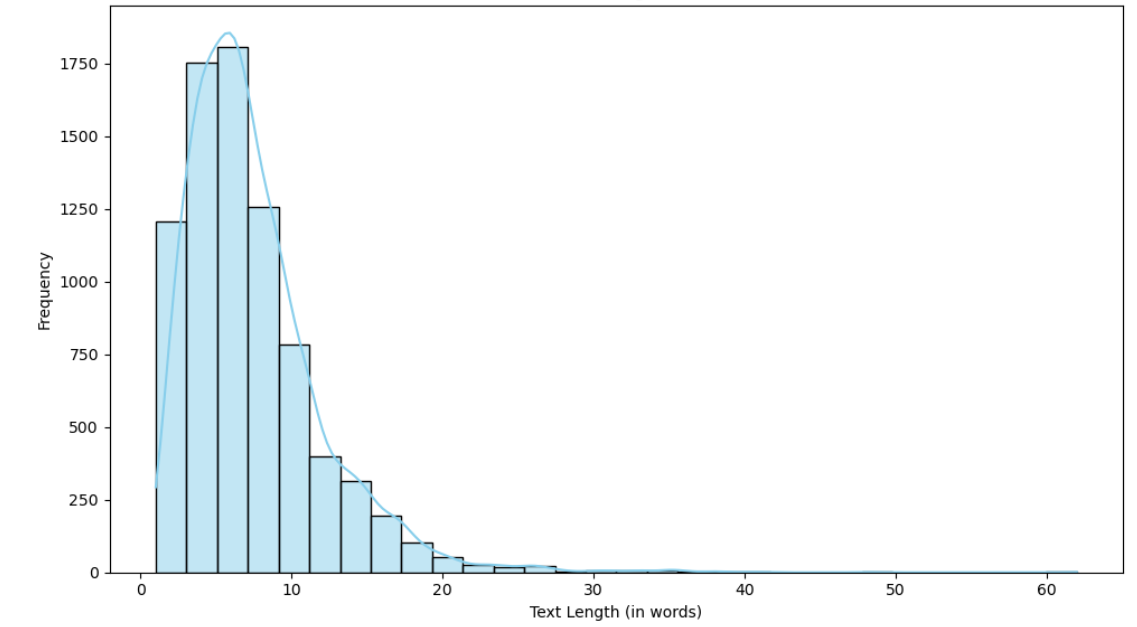
\includegraphics[width=.55\linewidth]{distribution_of_text_lengths.PNG}
    \caption{Distribution of Text Lengths in Annotations.}
    \label{fig:len}
\end{figure}
\end{frame}



\begin{frame}{Inconsistencies and Outliers}
    \begin{itemize}
        \item \textbf{No technical errors found:}
            \begin{itemize}
                \item No offsets before onsets
                \item No zero-duration annotations
            \end{itemize}
        \item Simple rule-based checks could automate this validation.
    \end{itemize}

\begin{itemize}
    \item \textbf{Descriptions with:}
    \begin{itemize}
        \item Zero words or just whitespace = errors
        \item One-word annotations = often uninformative
    \end{itemize}
\end{itemize}

\end{frame}

\end{document}